\documentclass[headsepline=true, abstracton]{scrartcl}
%\usepackage[ngerman]{babel}
\usepackage[utf8]{inputenc}
\usepackage[T1]{fontenc}
\usepackage{amssymb}
\usepackage{amsmath}
\usepackage{amsthm}
\usepackage{enumerate}
\usepackage{verbatim}
\usepackage[a4paper,text={140mm,215mm},centering,headsep=10mm,footskip=10mm]{geometry}
\usepackage[urlcolor=black,colorlinks=true,linkcolor=black,citecolor=black,bookmarks]{hyperref}
\usepackage{aliascnt}
\usepackage{lmodern}
\usepackage{mdwlist}
\usepackage{listings}
\usepackage[table,xcdraw]{xcolor}
\usepackage[activate]{pdfcprot}
\usepackage{graphicx}
\usepackage{slashed}
\usepackage{mathrsfs}
\usepackage{geometry}
\usepackage{float}
\usepackage{oldgerm}
\usepackage{setspace}
\usepackage{dsfont}
%\usepackage{mathtools}
\usepackage[all]{xy}
\usepackage{cite}
%\usepackage{amsmath}
\usepackage{amsfonts}
\usepackage{amssymb}
\usepackage{algorithm2e}
\usepackage{url}
\pagestyle{headings}
\newcommand{\myclearpage}{\clearpage}
\newcommand\independent{\protect\mathpalette{\protect\independenT}{\perp}}
\def\independenT#1#2{\mathrel{\rlap{$#1#2$}\mkern2mu{#1#2}}}
\newenvironment{gelaber}{}{}
\newenvironment{preamble}{}{}
\newcommand{\tostar}{\overset{*}{\lower0.5em\hbox{$\smash{\scriptscriptstyle\rightharpoonup}$}}}
\newtheorem{mydef}{Definition}
\newtheorem{bem}{Bemerkung}
\usepackage{tikz}
\newcommand\circlearound[1]{%
  \tikz[baseline]\node[draw,shape=circle,anchor=base] {#1} ;}
 
  
\begin{document}

\setcounter{section}{-1}

\renewcommand{\refname}{Bibliography}


\onehalfspacing
\setlength{\headsep}{15mm}


\thispagestyle{plain}

\title{\Large Analyzing the Supreme Court Citation Network}
\maketitle

\begin{abstract}
\noindent 
\end{abstract}


 \section*{Introduction}
 
 Coming...
 
 \section*{The Exponential Random Configuration Model}
Let $c(t)\in \{0,1\}^N$ be a vector indicating which Supreme Court case has been cited at time $t$, where $c_i(t)=1, i \in \{1, \dots , N\}$ indicates that the $i$th case has been cited at time $t$ and $c_i(t)=0$ indicates that the $i$th case has not been cited at time $t$. Furthermore, let
$$\mathcal{C}_t(N)=\{c(t)\in \{0,1\}^N: c_i(t)\in \{0,1\} \}$$ 
be the set of all possible citation combinations at time $t$. Note that the cardinality of $\mathcal{C}_t(N)$ increases exponentially for every newly added case, which results in $2^N$ elements.\\
The probability function of the ERCM is defined as
\begin{equation}
P_{\theta}(c(t)~|~c(t-))=\cfrac{\exp\big(\theta^T\cdot h\big(c(t)~|~c(t-)\big)\big)}{\sum_{c(t)^*\in \mathcal{C}}\exp\big(\theta^T\cdot h\big(c(t)~|~c(t-)\big)\big)}
\label{ercm}
\end{equation}
where $c(t-)\in \{0,1\}^{N \times (t-1)}$ is a matrix that indicates which cases have been citing in each other before time $t$, $\theta \in \mathbb{R}^q$ is a q-dimensional vector of parameters,  $h: \mathcal{C}_t(N) \to \mathbb{R}^q ~, ~ \c(t) \to (h_1(c(t)), \dots , h_q(c(t)))^T$ is a q-dimensional vector of different statistics and $\kappa(\theta) := \sum_{c(t)^*\in \mathcal{C}}\exp(\theta^T\cdot h(c(t)|c(t-)))$ is a normalization constant that ensures that (\ref{ercm}) defines a probability function on $\mathcal{C}_t$.\\[0.3cm]

% Network Statistics
The generative process of a model are informed by
the decision regarding which network statistics $h(\cdot)$ are incorporated. We include the following statistics for the Supreme Court citation network:
$$h_{edges}:\mathcal{C}(N)\to \mathbb{R}~~~, ~~~c(t) \to \sum_{i=1}^Nc_i(t)$$
the number of citations made at time $t$. 
$$h_{outstar}:\mathcal{C}(N)\to \mathbb{R}~~~, ~~~c(t) \to \sum_{j<i}^Nc_i(t)\cdot c_j(t) \cdot \sqrt{\dfrac{(t-a)(t-a-b)}{t^2}}$$
the number of weighted outstars occuring at time $t$. We argue that it should be more likely to cite more recent cases than cases that have been decided further in the past. For the weight 
$$w(a,b):= \sqrt{\dfrac{(t-a)(t-a-b)}{t^2}}$$
we define $a$ and $b$ as the elapsed time since case $i$ and $j$ have been introduced to the network.
$$h_{triangle}:\mathcal{C}(N)\to \mathbb{R}~~~, ~~~c(t) \to \sum_{j<i}^Nc_i(t)\cdot c_j(t) \cdot
c_j(t_{-i}) \cdot w(a,b)$$
where $c_j(t_{-i})$ indicates whether case $j$ was cited at the time case $i$ was introduced into the network. Just as for the outstar statistic, we include a weighting factor to favor more recent cases. \\[0.3cm]


%Change Statistic
The individual entries $c_i(t)$ can be taken as a manifestation of single Bernoulli variables $C_i(t)$. This interpretation allows the following calculation regarding the conditional distribution of $C_i(t)$:
%
\begin{eqnarray*}
\dfrac{P_{\theta}(C_i(t)=1 ~|~ C_i(t)^c=c_i(t)^c)}{P_{\theta}(C_i(t)=0 ~|~ C_i(t)^c=c_i(t)^c)} &=&
\dfrac{P_{\theta}(C_i(t)=1 ~,~ C_i(t)^c=c_i(t)^c)}{P_{\theta}(C_i(t)=0 ~,~ C_i(t)^c=c_i(t)^c)} \\
                           &=&\dfrac{P_{\theta}(C(t)= c_i^+(t))}{P_{\theta}(C(t)=c_i^-(t))}\\
                           &=&\dfrac{\exp(\theta^T \cdot h(c_i^+(t)~|~c(t-)))}{\exp(\theta^T \cdot h(c_i^-(t)~|~c(t-)))}\\
                           &=& \exp(\theta^T \cdot (h(c_i^+(t)~|~c(t-)) - h(c_i^-(t)~|~c(t-)))
\end{eqnarray*}
%
This implies the following equation:
%
\begin{equation}
\text{logit}(P_{\theta}(C_i(t)=1 ~|~ C_i(t)^c=c_i(t)^c))= \theta^T \cdot (h(c_i^+(t)~~|c(t-)) - h(c_i^-(t)~|~c(t-)))
\label{Logit}
\end{equation}
In the equation above the following notations were used:
%
\begin{itemize}
\item $c_i^+(t)$ emerges from $c(t)$, while assuming $c_i(t)=1$
\item $c_i^-(t)$ emerges from $c(t)$, while assuming $c_i(t)=0$
\item The condition $C_i(t)^c=c_i(t)^c$ is short for: $C_j(t)=c_j(t)$ for all $j\in \{1,\dots,N\}$ with $i \neq j$
\item The expression $(\Delta c_i)(t):=h(c_i^+(t)~|~c(t-)) - h(c_i^-(t)~|~c(t-))$ is called the \textit{change statistic}. The $k$th component of $(\Delta c_i)(t)$ captures the difference between citation networks $c_i^+(t)$ and $c_i^-(t)$ on the $k$th integrated statistic in the model
\end{itemize}


\section*{Estimation}

% Pseudo Likelihood
\subsection*{Maximum Pseudo-Likelihood Estimator}
One can assume that the dyads are independent of each other, which means that
the random variables $C_i(t)$ inside the random vector $C(t)$ are independent of each other.
In this case, the equation (\ref{Logit}) reduces to
$$logit(P_{\theta}(C_i(t) = 1)) = \theta^T \cdot (\Delta c_i)(t)$$
This corresponds with the logistic regression approach, where the observations of
the dependent variables are simply edge values of the observed citation vector,
and the observations of the covariate values are given as the scores of every single
change statistic. Therefore, the resulting likelihood function is of the following form:
\begin{equation}
\text{lik}(\theta)= P_{\theta}(C(t)=c(t))= \prod_{i} \dfrac{ \exp \left(\theta^T \Delta(c_i)(t) \right)}{1+\exp \left(\theta^T \Delta(c_i)(t) \right)}
\label{PseudoLik}
\end{equation}

\subsection*{Maximum Likelihood Estimator}
The more rigorous technique is to estimate the parameters directly with the log-likelihood function derived from (\ref{ercm}), which has the following form:
%
\begin{equation}
\text{loglik}(\theta)=\theta^T \cdot h(c(t)| c(t-))-\log(\kappa(\theta))
\label{loglik}
\end{equation}
%
The problem resulting from estimating the parameters with (\ref{loglik}) is that the term
%
$$\kappa(\theta):= \sum_{c(t)^* \in \mathcal{C}(N)} \exp(\theta^T \cdot h(c(t)^*|c(t-)))$$ 
%
which sums up the weighted statistics of all possible binar vectors of length $N$, has to be evaluated. However, the cardinality of $\mathcal{C}(N)$ (\#$(\mathcal{C})=2^N$) is incredibly large and a direkt calculation of this sum is for already small $N$ not feasible. \\[0.3cm]
An solution for this limitation is based on the following consideration: Fix a vector of parameters $\theta_0 \in \Theta$ from the underlying parameter range $\Theta$ and compute for $\theta \in \Theta$ the expected value
%
\begin{eqnarray*}
\mathbb{E}_{\theta_0}\left[ \exp\left((\theta - \theta_0)^T \cdot \Gamma(C(t))\right) \right]&=& 
\sum_{c(t) \in \mathcal{C}(N)}\exp\left((\theta - \theta_0)^T \cdot \Gamma(c(t))\right)\cdot \mathbb{P}_{\theta_0}(C(t)=c(t))\\
&=& \sum_{c(t) \in \mathcal{C}(N)}\exp\left((\theta - \theta_0)^T \cdot \Gamma(c(t))\right)\cdot 
\frac{\exp(\theta_0^T \cdot \Gamma(c(t)))}{\kappa(\theta_0)}\\
&=& \frac{1}{\kappa(\theta_0)} \sum_{c(t) \in \mathcal{C}(N)}\exp\left(\theta^T \cdot \Gamma(c(t))\right)\\
&=&\frac{\kappa(\theta)}{\kappa(\theta_0)}
\end{eqnarray*}
%
This equation offers the following possibility: If one draws $L$ random vectors $c^{(1)}(t), \dots ,c^{(L)}(t)$ out of a distribution $\mathbb{P}_{\theta_0}$ appropriately, one gets with the law of big numbers and a big enough sample $L$ the following relation:
%
\begin{equation}
\frac{1}{L}\cdot \sum_{i=1}^{L}  \exp\left((\theta - \theta_0)^T \cdot \Gamma(c^{(i)}(t))\right)
~~\approx~~ \mathbb{E}_{\theta_0}\left[ \exp\left((\theta - \theta_0)^T \cdot \Gamma(C(t))\right) \right] = \frac{\kappa(\theta)}{\kappa(\theta_0)}
\label{konver}
\end{equation}
%
This approximate can then be used to approximate the log likelihood function.\\[0.4cm]
Next, we will discuss how a sufficient number of suitable drawings $c^{(1)}(t), \dots ,c^{(L)}(t)$ can be sampled from the distribution $\mathbb{P}_{\theta_0}$. \\
For this purpose, the Markov Chain Monte Carlo (MCMC) methods can be used.
\subsection*{Gibbs sampling for the ERCM}
To be able to compute the approximate likelihood function one needs a sufficiently large number of random vectors from the distribution $\mathbb{P}_{\theta_0}$. Snijders \cite{Snijders.2002b} introduces an approach to sample random networks for the ERGM framework by using \textit{MCMC methods}. We adapt this approach for sampling appropriate binary vectors for the ERCM. \\[0.4cm]
\textit{Gibbs sampling}\\
%Choose any vector $c^{(0)}(t) \in \mathcal{C}(N)$ (e.g. observed vector). Afterwards, the length $L$ of the respective sub-sequence is determined. For $k \in \{0,...,L-1\}$ execute the following steps recursively (here the vector in its $k$th iteration is denoted as $c^{(k)}(t)$):\\

\begin{algorithm}[H]
 Choose any vector $c^{(0)}(t) \in \mathcal{C}(N)$ (e.g. observed vector)\\
 \For{i in 1:N}{
  Compute $\pi:= \cfrac{\exp(\theta^T\cdot \Delta(c_i)(t))}{1+\exp(\theta^T\cdot \Delta(c_i)(t))}$\\
  Draw a random number Z from Bin(1,$\pi$)\\
  \eIf{Z=1}{
   set $c^{(k+1)}_i = 1$ and $c^{(k+1)}_j=c^{(k)}_j$, if $i\neq j$
   }{
   set $c^{(k+1)}_i = 0$ and $c^{(k+1)}_j=c^{(k)}_j$, if $i\neq j$
  }
 }
 Start all over using $c^{(k+1)}$\\[0.3cm]
 \caption{Simulation of vectors of $\mathbb{P}_\theta$ using Gibbs sampling}
\end{algorithm}
\vspace{0.5cm}
%\begin{enumerate}
%\item Randomly choose a number $i \in \{1,\dots, N\}$
%\item Compute using the likelihood the value 
%$$\pi:= \mathbb{P}_{\theta}(C_{i}(t)=1 | C_{i}^c(t)=(c_{i}^{(k)}(t))^c)=\cfrac{\exp(\theta^T\cdot \Delta(c_i)(t))}{1+\exp(\theta^T\cdot \Delta(c_i)(t))}$$
%\item Draw a random number $Z$ from Bin$(1, \pi)$. %If
%\begin{itemize}
%\item $Z=0$, define $c^{(k+1)}(t)$ via
%$$c_{p}^{(k+1)}(t)=\begin{cases}
%0& \text{if}~ p=i \\
%c_{p}^{(k)}(t) &\text{if}~ p \neq i 
%\end{cases}$$
%\item $Z=1$, define $c^{(k+1)}(t)$ via
%$$c_p^{(k+1)}(t)=\begin{cases}
%1& \text{if}~ p=i \\
%c_p^{(k)}(t) &\text{if}~ p \neq i 
%\end{cases}$$
%\end{itemize}
%\item Start at step 1 with $c^{(k+1)}(t)$.
%\end{enumerate}
\noindent Using the depicted algorithm, a sequence of random vectors $c^{(0)}(t),...,c^{(L)}(t)$ can be simulated. Since the orignial vector was chosen randomly and the first simulated vectors are very dependent on the chosen mvector (only one entry is changed per iteration!), usually the first $B$ vectors, where $N \ll B \ll L$, are discarded as the so called \textit{Burn-In}.
\subsection*{Metropolis Hastings for the ERCM}\label{networksimulation}
Choose any vector $c^{(0)}(t) \in \mathcal{C}(N)$ to start with (e.g., the observed vector). For $k \in \{0,...,L-1\}$ recursively proceed as follows:\\
\begin{enumerate}
\item Randomly choose a number $i\in \{1,\dots, N\}$
\item Compute, using the equation (\ref{Logit}) the value
$$\pi := \dfrac{\mathbb{P}_{\theta}(C_{i}(t) \neq c_{i}^{(k)}(t) ~| ~C_i(t)^c=c_i(t)^c)}{\mathbb{P}_{\theta}(C_{i}(t) = c_{i}^{(k)}(t) ~| ~C_i(t)^c=c_i(t)^c)}$$
\item Define $\delta:= \min\{1, \pi\}$ and draw a random number $Z$ from Bin$(1, \delta)$. If
\begin{itemize}
\item $Z=0$, let $c^{(k+1)}(t) := c^{(k)}(t)$ 
\item $Z=1$, define $c^{(k+1)}(t)$ as
$$c_{p}^{(k+1)}(t)=\begin{cases}
1-c_{p}^{(k)}(t)& \text{if}~ p=i \\
c_{p}^{(k)}(t) &\text{if}~ p \neq i 
\end{cases}$$
\end{itemize}
\item Start at step 1 with $c^{(k+1)}(t)$.
\end{enumerate}
The first $B \ll L$ vectors are discarded as Burn-In.


 \section*{Results}
  \subsection*{Descriptive Results}
 The supreme court citation network from $1937 - 2005$ consists of $8817$ cases which got voted at 2116 different time points. The network has a total of $93,263$ ties, of which 452 are mutual. The number of triangles in the network is $211,855$. The in- and outdegree distribution is visualized in figures \ref{indegree_dist} and \ref{outdegree_dist}. The maximum indegree is $190$ and the maximum outdegree is $159$.
 

\begin{figure}
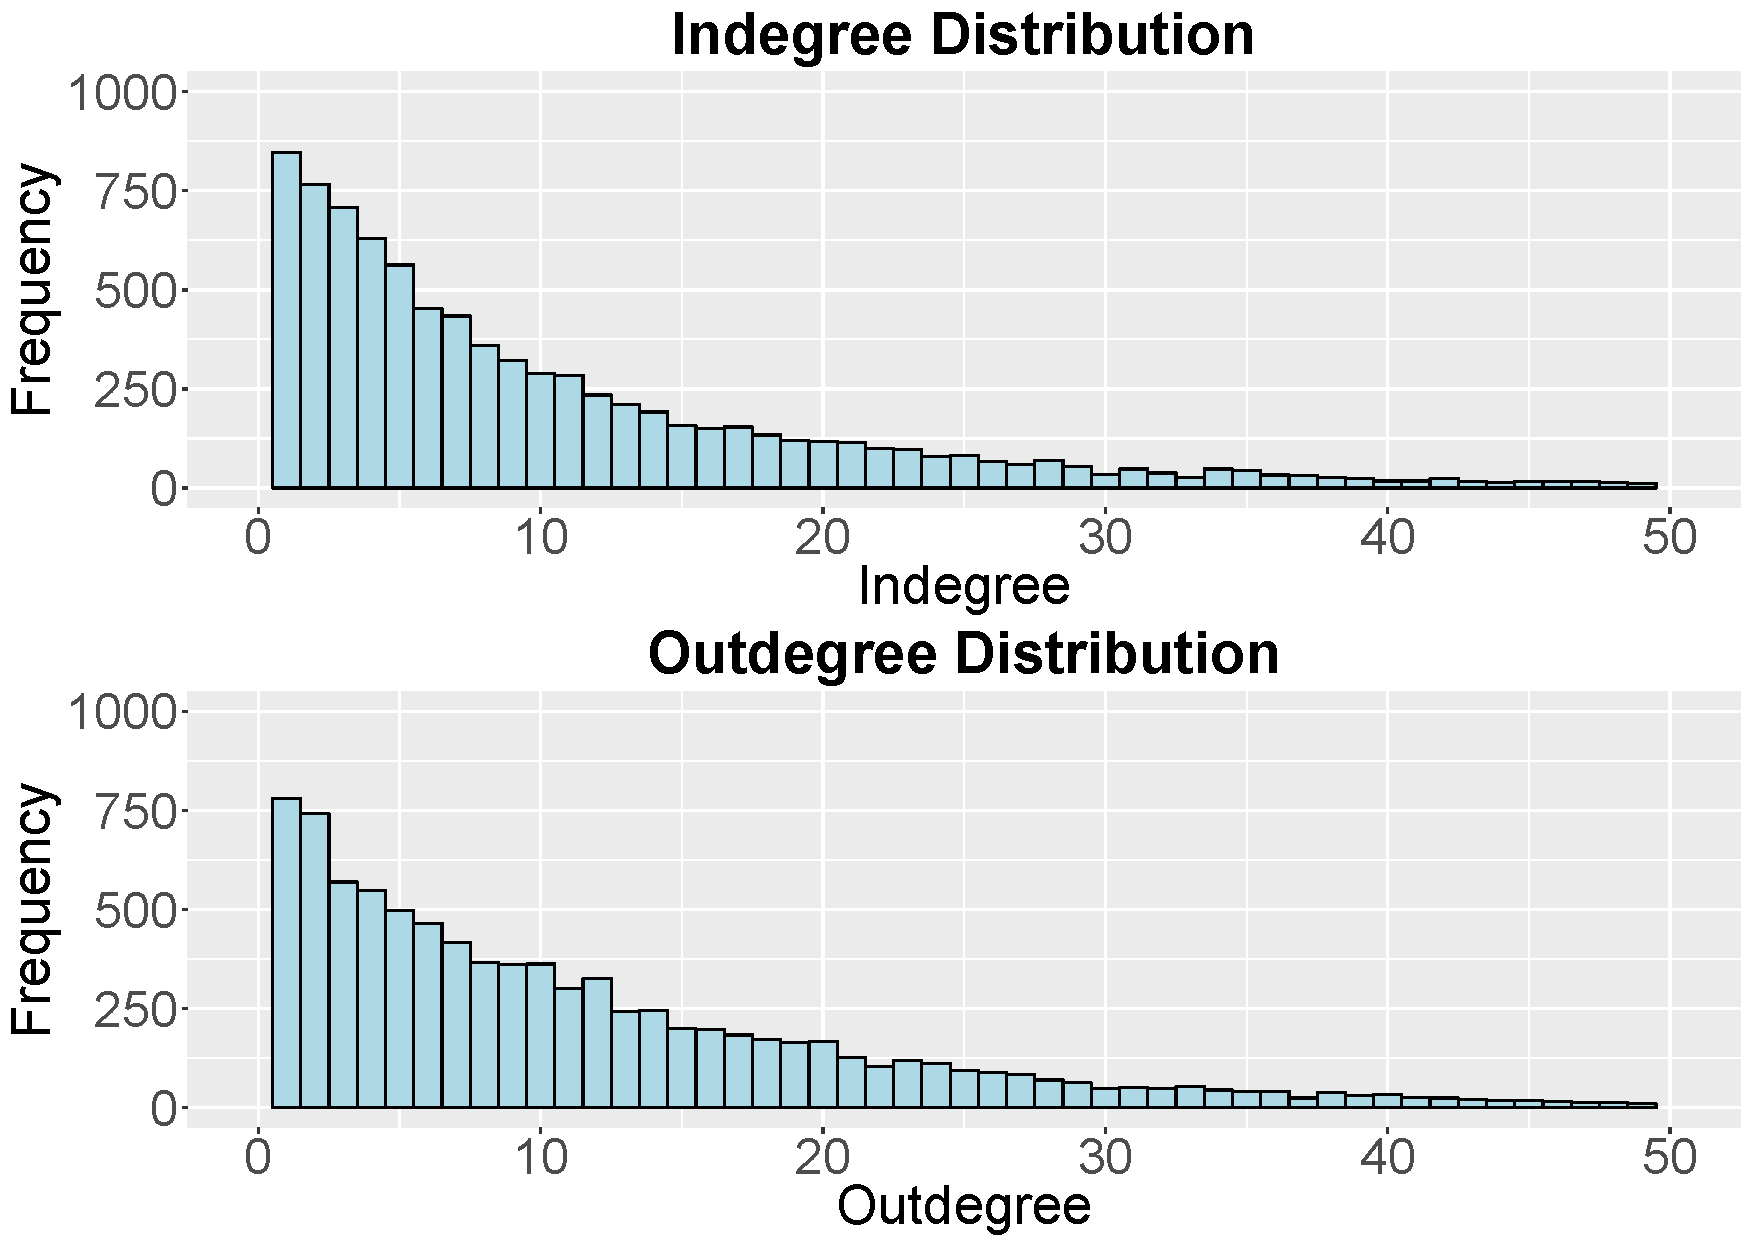
\includegraphics[scale=0.5]{degree_distribution}
\caption{The in- and outdegree distribution of the Supreme Court Citation Network from 1937 - 2005. There are cases with an indegree >50, but they are not captured in this figure.}
 \label{degree_dist}
\vspace{-.25cm}
\end{figure}

   
\subsection*{Inferential Results}

\begin{table}[]
\centering
\begin{tabular}{|
>{\columncolor[HTML]{C0C0C0}}l |l|l|l|}
\hline
{\color[HTML]{333333} } & \cellcolor[HTML]{C0C0C0}{\color[HTML]{333333} Estimate} & \cellcolor[HTML]{C0C0C0}{\color[HTML]{333333} Lower Bound} & \cellcolor[HTML]{C0C0C0}{\color[HTML]{333333} Upper Bound} \\ \hline
Edges                   & -5.445                                                 & -5.514                                                     & -5.296                                                     \\ \hline
Instar(2)               & 0.033                                                   & 0.028                                                      & 0.040                                                      \\ \hline
Outstar(2)              & 0.015                                                   & -0.001                                                      & 0.016                                                      \\ \hline
Mutual                  & 4.717                                                   & 4.093                                                 & 5.422                                                      \\ \hline
Triangle                & 1.337                                                   & 1.251                                                      & 1.475                                                      \\ \hline
MQ Score                & -0.009                                                   & -0.035                                                      & 0.087                                                      \\ \hline
Same Issue Area         & 1.205                                                   & 1.064                                                      & 1.237                                                      \\ \hline
Year Difference         & -0.076                                                   & -0.101                                                     & -0.072                                                          \\ \hline
\end{tabular}
\caption{Bootstrappped MPLE Results for the timep period when Fred M. Vinson was chief justice.}
\label{bootMPLE_vinson}
\end{table}   
 

\begin{table}[]
\centering
\begin{tabular}{|
>{\columncolor[HTML]{C0C0C0}}l |l|l|l|}
\hline
{\color[HTML]{333333} } & \cellcolor[HTML]{C0C0C0}{\color[HTML]{333333} Estimate} & \cellcolor[HTML]{C0C0C0}{\color[HTML]{333333} Lower Bound} & \cellcolor[HTML]{C0C0C0}{\color[HTML]{333333} Upper Bound} \\ \hline
Edges                   & -5.042                                                 & -5.107                                                     & -4.952                                                     \\ \hline
Instar(2)               & 0.028                                                   & 0.026                                                      & 0.033                                                      \\ \hline
Outstar(2)              & 0.018                                                   & 0.017                                                      & 0.022                                                      \\ \hline
Mutual                  & 3.158                                                   & 1.469                                                 & 3.508                                                      \\ \hline
Triangle                & 1.500                                                   & 1.391                                                      & 1.506                                                      \\ \hline
MQ Score                & -0.106                                                   & -0.142                                                      & -0.067                                                      \\ \hline
Same Issue Area         & 1.334                                                   & 1.274                                                      & 1.378                                                      \\ \hline
Year Difference         & -0.031                                                   & -0.040                                                     & -0.029                                                          \\ \hline
\end{tabular}
\caption{Bootstrappped MPLE Results for the timep period when Earl Warren was chief justice.}
\label{bootMPLE_vinson}
\end{table}


\begin{table}[]
\centering
\begin{tabular}{|
>{\columncolor[HTML]{C0C0C0}}l |l|l|l|}
\hline
{\color[HTML]{333333} } & \cellcolor[HTML]{C0C0C0}{\color[HTML]{333333} Estimate} & \cellcolor[HTML]{C0C0C0}{\color[HTML]{333333} Lower Bound} & \cellcolor[HTML]{C0C0C0}{\color[HTML]{333333} Upper Bound} \\ \hline
Edges                   & -3.961                                                 & -4.036                                                     & -3.911                                                     \\ \hline
Instar(2)               & 0.016                                                   & 0.014                                                      & 0.037                                                      \\ \hline
Outstar(2)              & 0.004                                                   & 0.003                                                      & 0.006                                                      \\ \hline
Mutual                  & 2.528                                                   & 1.193                                                 & 3.007                                                      \\ \hline
Triangle                & 1.372                                                   & 1.248                                                      & 1.341                                                      \\ \hline
MQ Score                & -0.084                                                   & -0.096                                                      & -0.054                                                      \\ \hline
Same Issue Area         & 0.957                                                   & 0.917                                                      & 0.995                                                      \\ \hline
Year Difference         & -0.017                                                   & -0.019                                                     & -0.015                                                          \\ \hline
\end{tabular}
\caption{Bootstrappped MPLE Results for the timep period when Warren E. Burger was chief justice.}
\label{bootMPLE_vinson}
\end{table}   
 


 
\begin{table}[]
\centering
\begin{tabular}{|
>{\columncolor[HTML]{C0C0C0}}l |l|l|l|}
\hline
{\color[HTML]{333333} } & \cellcolor[HTML]{C0C0C0}{\color[HTML]{333333} Estimate} & \cellcolor[HTML]{C0C0C0}{\color[HTML]{333333} Lower Bound} & \cellcolor[HTML]{C0C0C0}{\color[HTML]{333333} Upper Bound} \\ \hline
Edges                   & -3.618                                                 & -3.666                                                     & -3.539                                                     \\ \hline
Instar(2)               & 0.015                                                   & 0.014                                                      & 0.016                                                      \\ \hline
Outstar(2)              & 0.001                                                   & -0.002                                                      & 0.004                                                      \\ \hline
Mutual                  & 9.667                                                   & 8.218                                                 & 11.253                                                      \\ \hline
Triangle                & 1.546                                                   & 1.433                                                      & 1.551                                                      \\ \hline
MQ Score                & -0.007                                                   & -0.023                                                      & 0.032                                                      \\ \hline
Same Issue Area         & 0.852                                                   & 0.751                                                      & 0.846                                                      \\ \hline
Year Difference         & -0.016                                                   & -0.018                                                     & -0.014                                                          \\ \hline
\end{tabular}
\caption{Bootstrappped MPLE Results for the timep period when William Rehnquist was chief justice.}
\label{bootMPLE_vinson}
\end{table}  
 
   
\newpage


\bibliography{bib} 
\bibliographystyle{plain}


\end{document}
